% 초안 v3 — XeLaTeX + kotex 로 컴파일 (Overleaf: Compiler = XeLaTeX). 내용은 DRAFT_v3.md 와 같다.
% 숫자는 docs/RESULTS_LOG.md 의 번호(R-xxx)가 있는 것만 썼다. 없는 숫자는 [R-xxx 예정] 으로 비워 둔다.
\documentclass[10pt,a4paper]{article}
\usepackage{kotex}
\IfFontExistsTF{Noto Sans CJK KR}{\setmainhangulfont{Noto Sans CJK KR}}{\setmainhangulfont{Malgun Gothic}}   % Overleaf: Noto, 윈도우: 맑은 고딕
\usepackage[margin=20mm]{geometry}
\usepackage{amsmath,amssymb,amsthm}
\usepackage{booktabs,array,multirow}
\usepackage{graphicx}
\usepackage{algorithm,algpseudocode}
\usepackage[colorlinks=true,linkcolor=blue,citecolor=blue,urlcolor=blue]{hyperref}
\usepackage{xcolor}
\newcommand{\todo}[1]{\textcolor{red}{[#1]}}
\newtheorem{proposition}{명제}
\newtheorem{definition}{정의}
\graphicspath{{./}}

\title{균형 장부: 연합 언러닝에서 삭제로 깨어나는 백도어를\\학습 중 상쇄 연합으로 찾아 걷어내기}
\author{(저자)}
\date{초안 v3, 2026-10-13}

\begin{document}
\maketitle

\begin{abstract}
연합 언러닝(federated unlearning, FU)은 클라이언트가 자기 기여의 삭제를 요청하면 서버가 저장된 기여로 모델에서 그 몫을 걷어내는 절차다. 최근 공격(FUBA, BadFU)은 이 절차를 역이용한다. 공격자 일부(운반자)는 백도어를 심고, 다른 한 명(위장자)은 같은 입력에서 반대 방향으로 밀어 학습 중 모델을 깨끗하게 보이게 한 뒤, 위장자가 삭제를 요청하면 백도어가 깨어난다. 우리는 이 공격이 ``같은 입력 영역에 모순된 지도를 공급해 평균을 0으로 만드는 것''이며, 그 결과 정상 학습에는 없는 구조---한 클래스를 여럿이 밀고 한 명이 그만큼 되미는 \emph{상쇄 연합}---를 반드시 남긴다는 것을 보인다. 이를 재는 \emph{균형 장부}(Balance Ledger)를 제안한다. 서버는 라운드마다 참여자의 갱신이 공개 입력 위에서 각 클래스를 미는 양을 누적하고, 클래스마다 헤지 비율·음의 다리·양의 다리 집합을 계산해, 양의 다리가 여럿이고 한 명이 독식하지 않는 균형 클래스가 지속되면 경보를 울린다. 경보는 타깃 클래스, 위장자, 운반자 집합, 되감을 라운드를 함께 준다. 대응은 그 라운드로 되감고 연합을 제외한 채 이어 학습하는 것이다. FUBA 논문 설정(클라이언트 20, 악성 5, 100 라운드, 참여 0.4, IID·non-IID 각 3 시드)에서 장부는 6/6 궤적에서 11--16 라운드에 경보를 내고 위장자와 운반자 넷을 오탐 없이 특정했으며, 클래스 소유자(한 클래스의 90\%를 가진 정상 클라이언트)를 한 번도 제외하지 않았다. 연합을 제외한 재학습은 ASR 0.5--0.6\%, 정확도 99\%에 닿는다. 갱신 하나의 크기·방향을 보는 기존 방어는 소유자를 같이 잡거나 운반자를 가장 정상으로 보며, 요청 시점에 빼 보는 심사는 모델 생성이 필요하고 더 늦다.
\end{abstract}

\section{서론}
\paragraph{문제.}
연합학습(FL)에서 클라이언트는 데이터 대신 갱신을 보내고 서버는 평균을 낸다. 삭제권(GDPR 17조)을 지키려면 서버는 특정 클라이언트의 몫을 모델에서 걷어내야 하고, 이를 위해 FedEraser 류의 서버는 라운드별 기여 $U_j^t$를 저장한다. 이 저장과 삭제가 새 공격면이 된다. Zhang 등~\cite{zhang2023}, Liu 등~\cite{liu2024}, UBA-Inf~\cite{ubainf}, BadFU~\cite{badfu}, FUBA~\cite{fuba}는 모두 같은 구조다. 운반자 집합 $A$는 트리거 입력을 타깃 클래스로 보내는 성분을 심고, 위장자 $S$는 같은 입력에서 그 성분을 되미는 성분을 심는다. 학습이 끝난 모델 $\theta_T$는 깨끗하다(ASR 3--8\%, 표~\ref{tab:attack}). 위장자가 삭제를 요청해 서버가 $U_S$를 걷어내면 되밀던 힘이 사라져 백도어가 깨어난다(ASR 46--93\%). 서버가 요청을 정확히 이행할수록 공격은 더 잘 된다: 운반자가 남은 채 처음부터 재학습해도 백도어 모델이 나온다($K=8$ 예비, ASR 30--44\%).

\paragraph{기존 방어의 틈.}
FL 방어는 갱신 \emph{하나}의 성질(노름, Krum 거리, 서버 기준과의 코사인, 출력층 에너지)이나 갱신들의 \emph{닮음}(FoolsGold)을 본다. 이 공격에서 위장자는 크기가 커서 크기 기준에 걸리지만, 한 클래스를 많이 가진 정상 클라이언트(소유자)도 같이 걸린다(소유자 $z$ 3.8--65, 표~\ref{tab:baselines}). 운반자는 방향이 가장 중심에 있어(20명 중 평균 순위 18.5) 어떤 단일 갱신 기준으로도 보이지 않는다. FU 전용 방어(MASA의 언러닝 손실, SubID의 부분공간 잔차)는 요청자 한 명의 갱신만 보므로 두 몫의 \emph{관계}인 상쇄를 보지 못한다. 요청 시점에 조금 빼 보는 심사는 위장자만 잡지만(flow $z$, 소유자 $z$ 0.0) 요청이 올 때까지 기다려야 하고 라운드마다 모델을 만들어야 한다.

\paragraph{핵심 관찰.}
공격 논문들은 잠복을 ``손실항 A가 손실항 B를 상쇄한다''는 한 문장으로만 설명한다. 우리는 이것을 \emph{모순 지도의 평균화}로 본다. 선형화(경험적 NTK) 아래 같은 입력 영역에 반대 라벨이 들어오면 잔차 부호가 반대라 커널 회귀가 라벨 평균을 배우고, 한쪽 공급자를 빼면 평균이 뒤집힌다~\cite{hayase2022}. 이 평균화는 공급자별로 분해되고, 그 분해가 라운드별 갱신이 공개 입력 위에서 각 클래스를 미는 양 $P_j(c)$다. 백도어가 잠복하려면 $\sum_j P_j(c^*)\approx 0$이면서 $|P_S(c^*)|\approx|\sum_{j\in A}P_j(c^*)|$가 커야 한다. 이것은 정상 학습에는 없는 관계 구조---여럿이 밀고 한 명이 되미는 \emph{상쇄 연합}---이며, 공격이 이것을 피하려면 백도어를 약하게 하거나(실패) 되밀기를 여럿에 나누어야 한다(\S\ref{sec:analysis}).

\paragraph{기여.}
\begin{enumerate}
\item 삭제로 깨어나는 백도어의 기제를 ``모순 지도의 평균화''로 정식화하고, 그 필요조건이 학습 중 장부에서 관찰 가능한 관계 불변량(상쇄 연합)임을 보인다(\S\ref{sec:obs}, \S\ref{sec:analysis}).
\item 균형 장부: 역할·라벨·트리거 정보 없이, 라운드당 참여자 수만큼의 순전파로 상쇄 연합을 찾고 타깃 클래스·위장자·운반자·되감기 라운드를 함께 내는 학습 중 방어(\S\ref{sec:method}).
\item 탐지가 준 정보를 그대로 쓰는 대응: 되감기 + 연합 제외 이어 학습. 요청 시점에는 같은 장부를 저장 갱신에 사후 적용한다(\S\ref{sec:response}).
\item FUBA 논문 설정 6 궤적에서 6/6 경보(11--16 라운드), 위장자·운반자 정밀도·재현율 1.0, 소유자 오제외 0, 제외 후 ASR 0.5--0.6\%. 갱신 크기·방향·요청 심사·null-space·학습 중 감사·참여 회귀 등 9 계열 36 점수와 같은 궤적에서 비교(\S\ref{sec:eval}).
\end{enumerate}

\section{배경과 관련 연구}
\paragraph{연합 언러닝.}
서버는 $\theta_t=\theta_{t-1}+\frac{1}{|P_t|}\sum_{j\in P_t}u_j^t$로 갱신하고($P_t$: 참여자), $U_j^t=u_j^t/|P_t|$를 저장한다. 요청 $k$에 FedEraser~\cite{federaser}는 저장 기여로 보정 재구성, 빼기 연산자는 $\theta_T-\rho\sum_t U_k^t$, 재학습은 $k$를 뺀 채 처음부터 학습한다.

\paragraph{삭제로 깨어나는 백도어.}
Zhang 등~\cite{zhang2023}은 오염 표본과 완화 표본(같은 트리거, 원래 라벨)을 함께 학습시키고 완화 표본의 삭제를 요청한다. Liu 등~\cite{liu2024}은 ``잠복 트리거''를 언러닝으로 ``증폭''한다. UBA-Inf~\cite{ubainf}는 위장 표본을 오염 표본에 대한 영향이 반대가 되도록 영향 함수로 최적화하며, 위장이 세면 백도어가 사라지고(vanishing) 약하면 미리 드러난다(exposure)고 보고한다---상쇄 크기를 정확히 맞춰야 한다는 뜻이다. BadFU~\cite{badfu}는 전역 갱신에 $p_1(\nabla L_{bd}+\nabla L_c)$가 들어가고 언러닝이 $\nabla L_c$를 빼면 백도어 기울기가 온전히 작용한다고 쓴다. FUBA~\cite{fuba}는 위장자를 ``Adv-defender''라 부르고 model-consistency 손실로 전역 모델이 깨끗해 보이도록 민다. 어느 논문도 잠복을 이론 대상으로 올리지 않았고, 방어는 요청 심사·사후 감시·DP를 제안하는 데 그친다.

\paragraph{FL 방어와 그 불변량.}
Krum~\cite{krum}(정상 기울기는 참 기울기 주위에 모인다), FLTrust~\cite{fltrust}(서버 뿌리 갱신과 방향이 맞는다), FLAME~\cite{flame}(백도어 갱신은 각도·크기가 정상 밀집 무리에서 벗어난다), DeepSight~\cite{deepsight}(오염 데이터는 덜 이질적이라 출력층 에너지가 몰린다), FoolsGold~\cite{foolsgold}(시빌은 서로 닮는다), FLDetector~\cite{fldetector}(정상 갱신은 헤세 예측과 일관된다), BaFFLe~\cite{baffle}(정상 전역 모델은 클래스별 오류가 점진적으로 변한다). 전부 갱신 하나의 성질 또는 갱신들의 닮음이다. ``갱신들이 서로 지운다''는 관계를 불변량으로 둔 방어는 없다. FU 전용: MASA~\cite{masa}, SubID~\cite{subid}, FedRecover~\cite{fedrecover}는 모두 요청자 한 명의 갱신을 본다.

\paragraph{상쇄를 설명하는 다른 틀.}
영향 함수~\cite{koh2017}, 섀플리 상호작용~\cite{grabisch}, 과제 산술~\cite{ilharco}(과제 벡터의 부정 = 잊기), 기울기 충돌~\cite{pcgrad}. 우리는 협력 게임의 ``연합은 더미(dummy)인데 구성원은 더미가 아니다''를 불변량의 이름으로 쓰고, 선형화를 기제 설명과 측정의 정당화에 쓴다. 매개변수 공간의 쌍별 코사인·부호 충돌은 우리 설정에서 위장자--운반자($+0.56$)와 위장자--정상($+0.60$)을 가르지 못해 통계로 쓰지 않는다(R-005).

\section{위협 모델}\label{sec:threat}
\paragraph{시스템.} $K$ 클라이언트, $T$ 라운드, 라운드당 참여율 $p$. 서버는 $\theta_{t-1}$, 참여자 집합 $P_t$, 갱신 $u_j^t$를 저장한다(FU 서버의 전제). 서버는 라벨 없는 공개 입력 $X_p$($|X_p|=500$, 시험 분포)를 가진다. 서버는 트리거, 타깃 클래스, 역할, 악성 수를 모른다.
\paragraph{공격자.} 악성 집합 $M\subset[K]$, $|M|<K/2$(논문 설정 5/20). $M$은 운반자 $A$와 위장자 $S$로 나뉜다. 목표: 학습 중 전역 모델은 트리거 입력에서 깨끗하고(잠복), $S$의 삭제 요청이 이행되면 트리거 입력이 타깃 $c^*$로 분류된다(활성화). 능력: 자기 데이터·손실·갱신을 임의로 정한다. 백도어는 한 타깃 클래스로 몰린다.
\paragraph{정상 클라이언트.} 자기 데이터로 정직하게 학습한다. 분포는 IID 또는 한 클라이언트가 한 클래스의 90\%를 갖는 non-IID(소유자). 정상 클라이언트도 삭제를 요청할 수 있고, 서버는 요청자의 의도를 심판하지 않는다.
\paragraph{방어 목표.} (G1) 요청 전에 상쇄 연합을 찾아 타깃·위장자·운반자를 특정한다. (G2) 정상 클라이언트(소유자 포함)를 제외하지 않는다. (G3) 삭제를 이행하면서 백도어를 없앤다. (G4) 라벨·트리거·역할 정보와 모델 생성 없이, 라운드당 순전파만으로 한다.

\section{핵심 관찰: 모순 지도의 평균화와 상쇄 연합}\label{sec:obs}
\paragraph{선형화.} $f_c(x;\theta)$를 클래스 $c$의 로그확률이라 하자. 라운드 $t$에 참여자 $j$의 가중 갱신 $U_j^t$가 공개 입력 $x$의 클래스 $c$에 주는 1차 변화는 $\langle U_j^t,\nabla_\theta f_c(x;\theta_{t-1})\rangle$이고, 전역 갱신의 변화는 참여자 합이다. 유한차분 $f_c(x;\theta_{t-1}+U_j^t)-f_c(x;\theta_{t-1})$는 순전파 한 번으로 이 양의 비선형 판을 준다.
\paragraph{밀기와 장부.}
\begin{equation}
P_j(c)=\sum_{t:\,j\in P_t}\ \operatorname{mean}_{x\in X_p}\big[f_c(x;\theta_{t-1}+U_j^t)-f_c(x;\theta_{t-1})\big].
\label{eq:push}
\end{equation}
정상 학습에서 $P_j(c)$는 $j$의 데이터가 $c$를 얼마나 가르쳤는지다. IID면 모두 비슷하고, 소유자는 자기 클래스에서 크게 양수다.
\paragraph{잠복의 필요조건.} 트리거 입력에서 성립하는 상쇄식 $J_{X^*}(U_S+\sum_{A}U_j)\approx 0$이 공개 입력 $X_p$에도 새면(FUBA의 consistency 손실은 전역 모델 전체를 깨끗한 모델 쪽으로 밀므로 새는 것이 관찰된다, R-012) 장부에는
\begin{equation}
P_S(c^*)\approx-\sum_{j\in A}P_j(c^*),\qquad |P_S(c^*)|\gg \text{정상의 }|P_j(c^*)|
\end{equation}
가 남는다. 즉 클래스 $c^*$에서 (i) 합은 0에 가깝고 (ii) 개별은 크며 (iii) 음의 다리는 한 명이고 (iv) 양의 다리는 여럿이다. 이 넷을 함께 갖는 클래스를 \emph{상쇄 연합이 있는 클래스}라 부른다.
\paragraph{정상에서는 왜 없는가.} 정상 클라이언트들의 $P_j(c)$는 같은 부호로 더해지거나(IID) 소유자 한 명이 크게 양수이고 나머지는 작다(non-IID). ``한 명이 크게 음수이고 그 크기가 여럿의 양수 합과 같다''는 데이터 분포의 차이로는 생기지 않는다---그것은 다른 사람들의 가르침을 \emph{되돌리는} 것이고, 정직한 학습은 남의 가르침을 되돌릴 이유가 없다. 실측(R-012, 그림~\ref{fig:push}): 위장자 $P(c^*)$ $-29.7\ldots-39.4$(6/6 최솟값), 운반자 $+3.3\ldots+16.3$, 정상 $-3.9\ldots+4.9$, 소유자 $+0.2\ldots+3.8$.
\begin{figure}[t]\centering
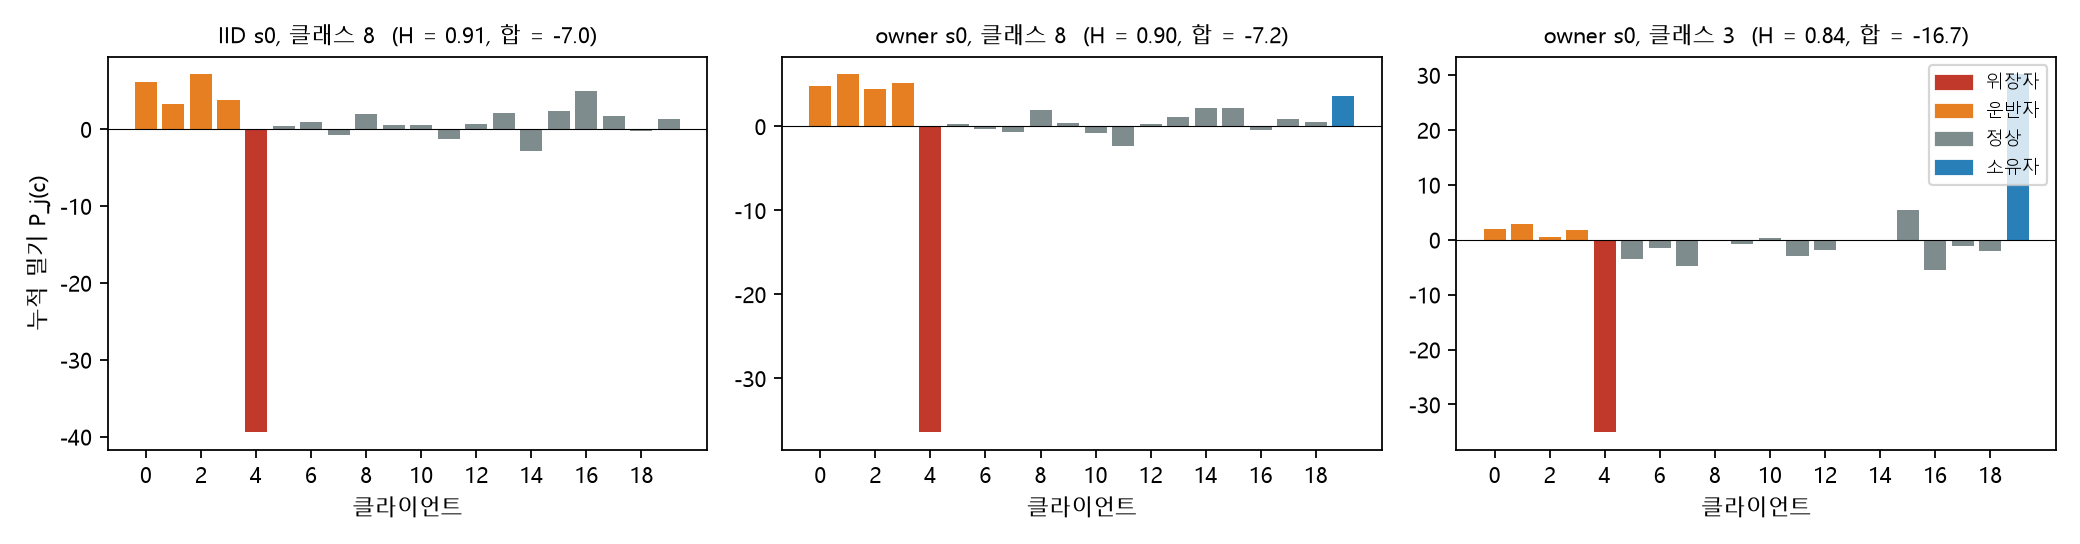
\includegraphics[width=\linewidth]{fig_push_bar.png}
\caption{학습 끝의 누적 밀기 $P_j(c)$. 왼쪽·가운데: 타깃 클래스 8---운반자 넷(주황)이 밀고 위장자(빨강)가 되민다($H$ 0.91 / 0.90). 오른쪽: owner 조건의 소유 클래스 3---소유자(파랑) 한 명이 밀고 위장자가 되민다($H$ 0.84): 음의 다리는 같지만 양의 다리가 한 명이다.}
\label{fig:push}
\end{figure}
\paragraph{소유자와의 구분.} non-IID 조건에서 위장자는 소유자가 가르친 클래스 3도 되민다(소유자 $+30$, 위장자 $-35$). 따라서 클래스 3도 ``합은 0, 음의 다리 한 명''이다. 차이는 양의 다리다: 클래스 8은 운반자 넷이 비슷하게(최대 몫 0.31--0.54), 클래스 3은 소유자 한 명이 거의 전부(몫 $>0.6$) 민다. 공모는 여럿이 나눠 미는 것이고 정상 큰손은 한 명이 미는 것이다. 이 구분이 판정 규칙의 넷째 조건이 된다.

\section{균형 장부}\label{sec:method}
\paragraph{불변량.} 정상 학습에서는 어떤 클래스에도 상쇄 연합((i)--(iv))이 없다. 삭제로 깨어나는 백도어는 타깃 클래스에 반드시 하나 만든다.
\paragraph{점수(라운드 $t$, 참여자 $j$, 순전파 1회).}
\begin{align}
H(c)&=1-\Big|\textstyle\sum_j P_j(c)\Big|\Big/\textstyle\sum_j|P_j(c)| \quad\text{(헤지 비율)}\\
\mathrm{neg}(c)&=\arg\min_j P_j(c),\qquad z_{\mathrm{neg}}(c)=\frac{P_{\mathrm{neg}}(c)-\operatorname{med}_jP_j(c)}{\operatorname{MAD}_jP_j(c)}\\
\mathrm{Pos}(c)&=\{j\neq\mathrm{neg}(c): z_j(c)>\kappa\},\qquad \mathrm{share}(c)=\frac{\max_{j\in\mathrm{Pos}(c)}P_j(c)}{\sum_{j\in\mathrm{Pos}(c)}P_j(c)}
\end{align}
장부에 $n_{\min}$ 라운드 이상 참여한 클라이언트만 다리 후보다.
\paragraph{영분포와 판정.} 영분포는 같은 클래스의 나머지 클라이언트(MAD). 클래스 $c$는
\begin{itemize}
\item \textbf{공모} $\Leftrightarrow H(c)\ge h_0 \wedge z_{\mathrm{neg}}(c)\le-\tau \wedge |\mathrm{Pos}(c)|\ge m \wedge \mathrm{share}(c)\le s_0$;
\item \textbf{정상 큰손} $\Leftrightarrow$ 앞 둘을 만족하고 $|\mathrm{Pos}(c)|=1$ 또는 $\mathrm{share}(c)>s_0$ (손대지 않음);
\item \textbf{외톨이 음} $\Leftrightarrow$ 앞 둘만 만족하고 $\mathrm{Pos}(c)=\emptyset$ (보고만).
\end{itemize}
같은 클래스가 $r$ 라운드 연속 공모이면 \textbf{경보}. 판정은 $t\ge t_0$부터, 모든 클래스를 본다. 고정값: $h_0=0.8,\ \tau=3,\ \kappa=2,\ m=2,\ s_0=0.6,\ r=3,\ t_0=5,\ n_{\min}=2$(민감도 \S\ref{sec:sens}).
\paragraph{경보가 주는 것.} 타깃 $c^*$, 위장자 후보 $\mathrm{neg}(c^*)$, 운반자 후보 $\mathrm{Pos}(c^*)$(연속 판정 동안의 합집합), 되감기 라운드 $t_{\mathrm{back}}=$ 경보 전 $H(c^*)<h_0$였던 마지막 라운드.
\paragraph{대응.}\label{sec:response} 연합 $C=\{\mathrm{neg}(c^*)\}\cup\mathrm{Pos}(c^*)$. $\theta_{t_{\mathrm{back}}}$로 되감고 $C$를 제외한 채 남은 $T-t_{\mathrm{back}}$ 라운드를 이어 학습한다(저자 학습 코드 그대로, 시작 모델과 제외 목록만 다르다). 요청이 학습 후에 오는 경우: 저장된 $\{U_j^t\}$ 위에 같은 장부를 사후 계산해 같은 판정을 내리고, 연합을 제외한 재학습으로 요청을 이행한다.
\paragraph{비용.} 라운드당 $|P_t|+1$ 순전파(500장). 모델 생성·역전파·라벨·트리거 없음. 대응은 $T-t_{\mathrm{back}}$ 라운드 학습.

\begin{algorithm}[t]
\caption{균형 장부}
\begin{algorithmic}[1]
\Require 라운드마다 $(\theta_{t-1},P_t,\{U_j^t\})$, 공개 입력 $X_p$; 문턱 $h_0,\tau,\kappa,m,s_0,r,t_0$
\State $P\gets 0_{K\times C}$; $\mathrm{streak}\gets 0_C$
\For{$t=1..T$}
  \State $L_0\gets\operatorname{mean}_x f(x;\theta_{t-1})$
  \For{$j\in P_t$} $P_j\gets P_j+\operatorname{mean}_x f(x;\theta_{t-1}+U_j^t)-L_0$ \EndFor
  \If{$t<t_0$} \textbf{continue} \EndIf
  \For{$c=1..C$} $(H,\mathrm{neg},z_{\mathrm{neg}},\mathrm{Pos},\mathrm{share})$ 계산; $\mathrm{streak}[c]\gets$ 공모$(c)$ ? $\mathrm{streak}[c]+1$ : 0 \EndFor
  \If{$\exists c:\mathrm{streak}[c]\ge r$}
     \State $c^*\gets\arg\max_{\mathrm{streak}\ge r}H(c)$; $S\gets\mathrm{neg}(c^*)$; $A\gets\bigcup(\text{연속 판정 동안 }\mathrm{Pos}(c^*))$; $t_{\mathrm{back}}\gets\max\{t'<t: H_{t'}(c^*)<h_0\}$
     \State \Return 경보$(t,c^*,S,A,t_{\mathrm{back}})$ \Comment{대응: $\theta_{t_{\mathrm{back}}}$에서 $\{S\}\cup A$ 제외 이어 학습}
  \EndIf
\EndFor
\end{algorithmic}
\end{algorithm}

\section{분석}\label{sec:analysis}
\begin{proposition}[공격의 필요조건 $\Rightarrow$ 장부의 양성]
1차 선형화 아래, 학습 끝 모델이 트리거 입력 $X^*$에서 깨끗하고(잠복) $S$의 몫을 걷어내면 $X^*$가 $c^*$로 분류되며(활성화), 상쇄가 공개 입력 $X_p$에 비율 $\eta>0$으로 새면, 장부에서 $\sum_jP_j(c^*)=O(\text{정상 합})$, $P_S(c^*)\le-\eta\gamma$, $\sum_{j\in A}P_j(c^*)\ge\eta\gamma-O(\text{정상 합})$가 성립한다. 여기서 $\gamma$는 활성화에 필요한 로그확률 상승량이다. 따라서 $H(c^*)\to1$, $\mathrm{neg}(c^*)=S$, $\mathrm{Pos}(c^*)\supseteq A$.
\end{proposition}
\begin{proof}[증명 스케치] 잠복은 $X^*$ 위 합이 0, 활성화는 $S$의 몫이 $-\gamma$ 이하, 누출은 $X_p$로 $\eta$배 전달. 정상 합은 정상 클라이언트의 밀기 분산으로 유계. \end{proof}
\begin{proposition}[정상의 하한]
정상 클라이언트들의 $P_j(c)$가 독립이고 분산 $\sigma^2$이면, 어떤 클라이언트가 $z_{\mathrm{neg}}\le-\tau$를 만족할 확률은 MAD 기반 $z$의 꼬리로 유계이고, 동시에 $|\mathrm{Pos}|\ge2$, $\mathrm{share}\le s_0$, $H\ge h_0$일 확률은 그 곱보다 작다. 소유자는 자기 클래스에서 양수이므로 $\mathrm{neg}$가 되지 못하고, 소유자 클래스에서 양의 다리는 소유자 한 명($\mathrm{share}>s_0$)이다. \todo{공격 없는 궤적의 실측 R-015 예정}
\end{proposition}
\paragraph{적응 공격.} (a) 되밀기를 여러 위장자에 나누면 음의 다리가 집합이 된다---$\mathrm{Neg}(c)=\{z\le-\tau\}$로 두면 같은 규칙이 적용되며 위장자 2명 궤적에서 시험한다 \todo{R-016 예정}. (b) 되밀기를 약하게 하면 학습 중 ASR이 올라 잠복이 깨진다(UBA-Inf의 exposure). (c) 상쇄를 공개 입력에 새지 않게 트리거 영역에만 가두면($\eta\to0$) 장부는 보지 못한다---이것이 이 방어의 경계이며, 그 경우 요청 시점에 지울 입력을 포함한 집합에서 빼 보는 심사(R-009의 flow $z$)가 보완한다. (d) 운반자를 많이 두어 각자의 몫을 $\kappa$ 아래로 낮추면 $\mathrm{Pos}$가 비지만 합은 여전히 위장자를 상쇄해야 하므로 $H$와 $z_{\mathrm{neg}}$는 남는다(외톨이 음으로 보고됨; 운반자 특정은 못 한다).

\section{평가}\label{sec:eval}
\paragraph{설정.} FUBA 저자 코드 그대로. MNIST, LeNet, 클라이언트 20, 운반자 0--3, 위장자 4, 100 라운드(웜업 5), 참여율 0.4, 지역 에폭 50. 조건: IID, owner(클라 19가 클래스 3의 90\%). 시드 3(522--524). 공개 입력: 시험 집합 500장. 역할은 채점에만 쓴다. 연구 질문: RQ1 장부가 연합을 찾는가, 언제. RQ2 소유자·정상을 제외하지 않는가. RQ3 기존 계열과의 비교. RQ4 대응이 백도어를 없애는가. RQ5 문턱 민감도. RQ6 비용.

\begin{table}[t]\centering\small
\caption{공격 재현(R-006). 정확도/ASR(\%). 위장자를 전량 빼면 모델이 무너진다(정확도 9.7\%, R-007).}
\label{tab:attack}
\resizebox{\linewidth}{!}{%
\begin{tabular}{lllll}\toprule
 & 잠복 & 위장자 20\% 제거 & 정상 1명 제거 & 운반자 1명 제거\\\midrule
IID s0·s1·s2 & 98.8/7.4 · 98.7/3.1 · 98.6/4.8 & 68.7/92.6 · 97.6/46.2 · 86.6/82.3 & 97.8/3.9 · 96.5/2.4 · 94.8/4.9 & 98.3/0.6 · 98.1/0.6 · 97.3/0.6\\
owner s0·s1·s2 & 98.2/7.8 · 98.3/3.6 · 98.1/5.7 & 73.1/85.7 · 96.7/50.0 · 82.5/78.9 & 96.1/9.8 · 95.8/5.8 · 96.0/4.4 & 98.0/1.4 · 96.5/0.2 · 94.5/0.2\\
ASR 평균 (IID / owner) & 5.1$\pm$1.8 / 5.7$\pm$1.7 & 73.7$\pm$19.9 / 71.5$\pm$15.5 & 3.7$\pm$1.0 / 6.7$\pm$2.3 & 0.6$\pm$0.0 / 0.6$\pm$0.6\\
\bottomrule\end{tabular}}
\end{table}

\begin{table}[t]\centering\small
\caption{RQ1·RQ2: 균형 장부(R-013; R-012). 역할 정보 없음.}
\label{tab:ledger}
\resizebox{\linewidth}{!}{%
\begin{tabular}{lll}\toprule
 & IID (3 시드) & owner (3 시드)\\\midrule
경보 라운드 / 99 & 13.0$\pm$1.6 (13, 15, 11) & 14.0$\pm$2.2 (16, 15, 11)\\
경보 클래스 $=c^*$(8) & 3/3 & 3/3\\
$\mathrm{neg}(c^*)=$ 위장자 4 & 3/3 & 3/3\\
$\mathrm{Pos}(c^*)=$ 운반자 \{0,1,2,3\}: 정밀도/재현율 & 1.0/1.0 & 1.0/1.0\\
소유자 19 $\in$ 제외 목록 & --- & 0/3\\
학습 끝 장부의 오경보 클래스 & 0/3 & 0/3\\
$H(c^*)$: 경보 시 $\to$ 끝 & 0.86$\pm$0.04 $\to$ 0.91$\pm$0.02 & 0.89$\pm$0.01 $\to$ 0.90$\pm$0.01\\
$z_{\mathrm{neg}}(c^*)$: 경보 시 $\to$ 끝 & $-8.2\pm1.8\to-18.4\pm1.7$ & $-6.5\pm2.4\to-17.7\pm1.1$\\
$c^*$ 아닌 클래스의 최대 $H$(끝) & 0.81$\pm$0.03 & 0.84$\pm$0.01\\
$\mathrm{share}(c^*)$(운반자 최대 몫) & 0.41$\pm$0.09 & 0.39$\pm$0.11\\
$t_{\mathrm{back}}$ & 10, 12, 7 & 13, 12, 7\\
$P(c^*)$ 끝: 위장자 / 운반자 / 정상 / 소유자 & $-39.4\ldots-29.7$ / $+3.3\ldots+16.3$ / $-3.1\ldots+4.9$ / --- & $-36.4\ldots-32.7$ / $+4.4\ldots+12.9$ / $-3.9\ldots+2.2$ / $+0.2\ldots+3.8$\\
순/총 밀기 $|\sum|/\sum|\cdot|$ ($c^*$) & 0.07--0.12 & 0.15--0.16\\
\bottomrule\end{tabular}}
\end{table}

\paragraph{RQ1·RQ2.} 표~\ref{tab:ledger}, 그림~\ref{fig:H}. 경보는 학습의 11--16\% 지점에 난다. 위장자는 모든 클래스의 음의 다리($z$ $-4\ldots-19$)이지만 양의 다리가 둘 이상이고 한 명이 독식하지 않는 클래스는 $c^*$뿐이다. owner 조건의 클래스 3은 정상 큰손으로 분류된다. 한 시드(owner s0)는 학습 끝에 정상 한 명이 클래스 3의 양의 다리에 더해져 $\mathrm{share}$ 조건이 없으면 공모로 걸린다($s_0=0.6$의 근거; 0.5는 IID s0의 $c^*$까지 깎는다). 다른 시드(owner s1)는 학습 끝에 소유자가 $c^*$의 $\mathrm{Pos}$에 들어오므로 제외 목록은 경보 시점의 것을 쓴다.
\begin{figure}[t]\centering
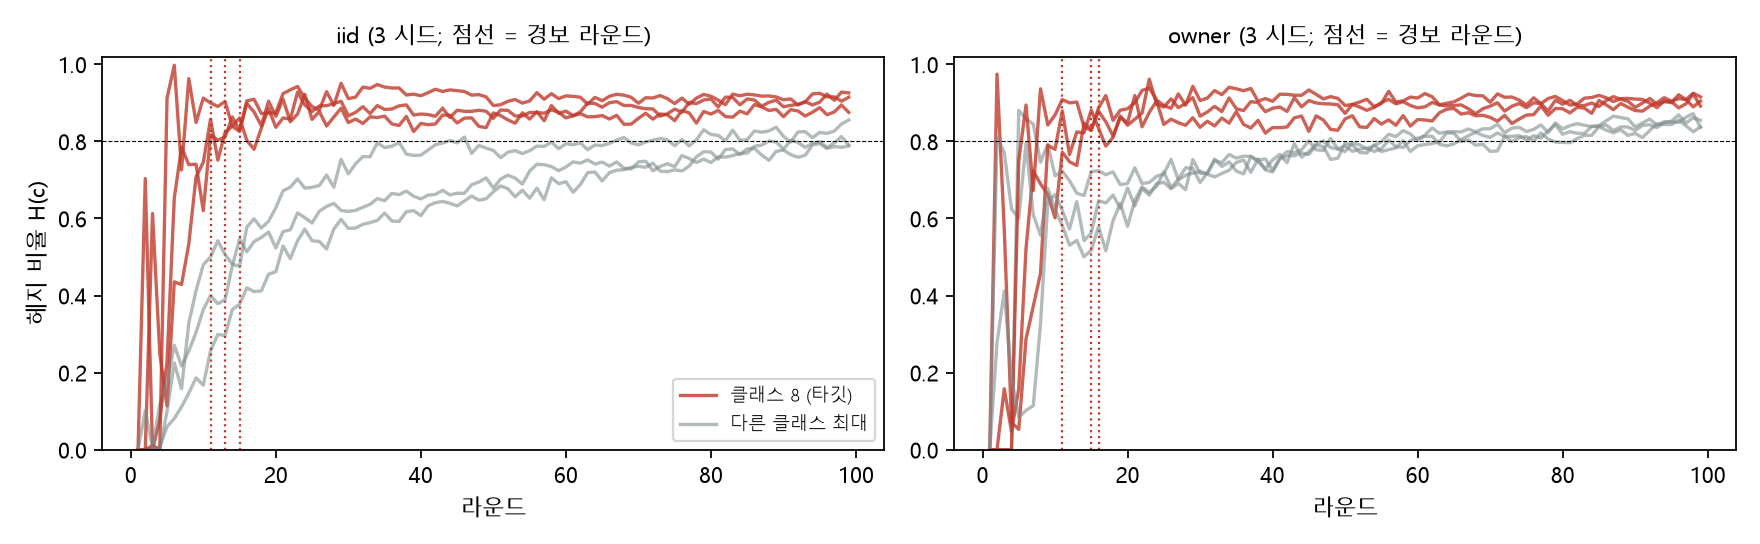
\includegraphics[width=\linewidth]{fig_H_curve.png}
\caption{라운드별 헤지 비율 $H(c)$. 타깃 클래스(빨강)는 10 라운드 안에 0.8을 넘고 끝까지 유지된다; 다른 클래스의 최대(회색)는 그 아래에 머문다. 점선은 경보 라운드(11--16).}
\label{fig:H}
\end{figure}

\begin{table}[t]\centering\small
\caption{RQ3: 기존 계열과의 비교(R-009; 같은 6 궤적, 36 점수 중 대표). 잡힘 = 위장자 순위 1인 시드 수; 소유자 $z$는 owner 조건.}
\label{tab:baselines}
\resizebox{\linewidth}{!}{%
\begin{tabular}{lccccc}\toprule
계열 (점수) & 잡힘 IID · owner & 소유자 $z$ & 운반자 평균 순위/20 & 모델 생성 & 시점\\\midrule
갱신 크기: 노름 · Krum · 총노출 & 3/3 · 3/3 & 3.8 · 6.8 · 2.8 & 18.5 & 없음 & 학습 중\\
갱신 방향: 중앙값 코사인 · 반상관 · 누적 코사인 & 0/3 · 0/3 & 1.9 · 2.0 · 1.0 & 2.6--4.9 & 없음 & 학습 중\\
요청 심사 절대 변화(20\% 빼기): 바뀐 답 · KL & 3/3 · 3/3 & 9.7 · 65.1 & 11--15 & 요청당 단계 수 & 요청 시\\
null-space 에너지 & 1/3 · 1/3 & $-9.9$ & 3--7 & 없음 & 요청 시\\
기능 효과: 타깃 몰림 · Fisher & 3/3 · 3/3 & $-1.8$ · 1.7 & 8--18 & 없음 & 요청 시\\
빼 보기 상대 기준(flow $z$, 20\%) & 3/3 · 3/3 & 0.0 & 3.0--3.7 & 요청당 $K$개 & 요청 시\\
학습 중 부분합 감사(라운드 74) & 3/3 · 3/3 & 0.0 & 2.9--3.0 & 라운드당 $K$개 & 학습 중\\
참여 자연 실험(참여 회귀) & 3/3 · 3/3 & $-1.5$ & 15.0--15.2 & 없음 & 학습 중\\
\textbf{균형 장부} & \textbf{3/3 · 3/3} & \textbf{제외 0/3} & \textbf{운반자 $=\mathrm{Pos}$ 4/4} & \textbf{없음} & \textbf{13--14 라운드}\\
\bottomrule\end{tabular}}
\end{table}
\paragraph{RQ3.} 표~\ref{tab:baselines}. 크기 기준은 소유자를 같이 잡고 운반자를 가장 정상으로 본다. 방향 기준은 운반자가 가장 중심이라 못 본다. 절대 변화 심사는 소유자 오탐. 위장자만 잡는 것은 상대 기준 빼 보기·기능 효과·부분합 감사·참여 회귀·장부이며, 이 중 운반자까지 특정하고 모델 생성 없이 가장 이른 것은 장부다.

\begin{table}[t]\centering\small
\caption{RQ4: 대응. ASR/정확도(\%), 요청자 = 위장자.}
\label{tab:remedy}
\resizebox{\linewidth}{!}{%
\begin{tabular}{llll}\toprule
처방 & IID & owner & 출처\\\midrule
정확한 언러닝 = 재학습, 운반자 남김 & 44.3$\pm$23.3 / 98.8 & 29.6$\pm$19.2 / 98.4 & $K=8$ 예비(R-001 설정)\\
증류 FU & 18--25 / --- & --- & R-007\\
빼기 + 재억제 증류 & 5.6$\pm$2.2 / 96.0$\pm$0.4 ($\alpha$ 0.09) & --- & R-008\\
해독제(짝 몫 투영 제거) & 실패 & 실패 & R-011\\
\textbf{연합 제외 재학습(처음부터)} & \textbf{0.5$\pm$0.1 / 99.0$\pm$0.0} & \textbf{0.6$\pm$0.2 / 98.9$\pm$0.0} & R-010\\
연합 제외, $t_{\mathrm{back}}=13$ 되감기 이어 학습 & 0.68 / 99.08 (노트북 1 시드) & \todo{R-014 예정} & R-014(예비)\\
연합 제외, 되감기 없이 경보 라운드 16에서 & 0.74 / 99.01 (노트북 1 시드) & \todo{R-014 예정} & R-014(예비)\\
(로컬 기준선) 연합 제외, 처음부터 & 0.31 / 99.07 (노트북 1 시드) & --- & R-014(예비)\\
\bottomrule\end{tabular}}
\end{table}
\paragraph{RQ4.} 표~\ref{tab:remedy}. 요청자를 완벽히 지우는 것(재학습)은 공격을 완성한다. 연합을 제외해야 ASR 0.5와 정확도 99가 동시에 나온다. 되감기 이어 학습과 경보 즉시 제외는 노트북 1 시드에서 둘 다 ASR $<1$, 정확도 99로 처음부터 재학습(0.31)과 같은 수준이며 라운드 13--16개를 아낀다 \todo{DISLAB 6 궤적 R-014 예정}.
\paragraph{RQ5: 문턱 민감도.}\label{sec:sens} (R-013, 노트북 IID 1 시드, 저장된 밀기로 재판정.) $h_0$ 0.7/0.8/0.9 $\to$ 경보 13/16/65 라운드, 목록 불변. $\tau=5\to$ 22 라운드. $\kappa=1.5\to$ 정상 1명이 $\mathrm{Pos}$에 섞임(정밀도 0.8); $\kappa=3\to$ 목록 불변. $r=1\to$ 7 라운드에 정상을 $\mathrm{neg}$로 오판; $r=5\to$ 18 라운드. $s_0$ 1.0/0.6/0.5 $\to$ 끝 장부 오경보 1/6 / 0/6 / $c^*$ 손상 1/6. 경보 시점은 문턱에 따라 움직이지만 누가 잡히는지는 $r\ge3,\kappa\ge2,s_0\in[0.6,1)$에서 변하지 않는다.
\paragraph{RQ6: 비용.} 장부: 라운드당 9 순전파 $\times$ 500장(논문 설정), 100 라운드 전체 1--2분(GPU 노트북). 요청 시점 심사(R-008): 요청당 모델 280개, 빼 보기 546회. 대응: 87--93 라운드 학습 vs 처음부터 100 라운드.

\section{한계와 남은 검증}
\begin{itemize}
\item \textbf{공격 없는 궤적의 오경보율}을 아직 재지 않았다(R-015 예정). 명제 2는 이 수치 없이는 주장이 아니다.
\item \textbf{누출 가정($\eta>0$).} 장부는 공개 입력에 새는 상쇄만 본다. FUBA의 consistency 손실은 샌다. BadFU의 위장 표본이 공개 입력에 새는지는 3 시드로 확인해야 한다. 새지 않으면 요청 시점 빼 보기(flow $z$)가 보완한다.
\item \textbf{위장자 여러 명, 다중 타깃.} $\mathrm{Neg}$ 집합 규칙은 코드에 있으나 궤적 실측 전이다.
\item 되감기 대응(R-014)의 6 궤적 실측과 집계 방어(Median·Multi-Krum·FLAME·FLDetector) 위 12 궤적은 실측 전이다.
\item 모델·데이터가 MNIST/LeNet이다(FUBA 논문 설정).
\end{itemize}

\section{결론}
삭제로 깨어나는 백도어는 모순 지도의 평균화이고, 그 평균화는 정상 학습에 없는 관계---여럿이 밀고 한 명이 되미는 상쇄 연합---를 학습 중 장부에 남긴다. 균형 장부는 라벨·트리거·역할·모델 생성 없이 그 연합을 11--16 라운드에 찾아 타깃·위장자·운반자·되감기 라운드를 주고, 연합을 걷어내면 삭제를 이행하면서 백도어가 사라진다.

\begin{thebibliography}{99}\small
\bibitem{zhang2023} Zhang et al. Backdoor attacks via machine unlearning (poison + mitigation samples). 2023.
\bibitem{liu2024} Liu et al. Backdoor attacks via machine unlearning. AAAI 2024.
\bibitem{ubainf} Huang et al. UBA-Inf: Unlearning activated backdoor attack with influence-driven camouflage. 2024.
\bibitem{badfu} BadFU: Backdoor federated learning through adversarial machine unlearning. 2025.
\bibitem{fuba} FUBA: Federated unlearning backdoor attack. 2025.
\bibitem{federaser} Liu et al. FedEraser: Enabling efficient client-level data removal from federated learning models. IWQoS 2021.
\bibitem{krum} Blanchard et al. Machine learning with adversaries: Byzantine tolerant gradient descent. NeurIPS 2017.
\bibitem{fltrust} Cao et al. FLTrust: Byzantine-robust federated learning via trust bootstrapping. NDSS 2021.
\bibitem{flame} Nguyen et al. FLAME: Taming backdoors in federated learning. USENIX Security 2022.
\bibitem{deepsight} Rieger et al. DeepSight: Mitigating backdoor attacks in federated learning through deep model inspection. NDSS 2022.
\bibitem{foolsgold} Fung et al. The limitations of federated learning in sybil settings. RAID 2020.
\bibitem{fldetector} Zhang et al. FLDetector: Defending federated learning against model poisoning attacks via detecting malicious clients. KDD 2022.
\bibitem{baffle} Andreina et al. BaFFLe: Backdoor detection via feedback-based federated learning. ICDCS 2021.
\bibitem{masa} MASA: Detecting malicious unlearning requests via unlearning loss. 2024.
\bibitem{subid} SubID: Subspace identification of malicious unlearning requests. INFOCOM 2026.
\bibitem{fedrecover} Cao et al. FedRecover: Recovering from poisoning attacks in federated learning using historical information. S\&P 2023.
\bibitem{hayase2022} Hayase and Oh. Few-shot backdoor attacks via neural tangent kernels. 2022.
\bibitem{koh2017} Koh and Liang. Understanding black-box predictions via influence functions. ICML 2017.
\bibitem{grabisch} Grabisch and Roubens. An axiomatic approach to the concept of interaction among players in cooperative games. 1999.
\bibitem{ilharco} Ilharco et al. Editing models with task arithmetic. ICLR 2023.
\bibitem{pcgrad} Yu et al. Gradient surgery for multi-task learning. NeurIPS 2020.
\end{thebibliography}
\end{document}
